\chapter{Implementation}\label{chap:implementation}

In this chapter, we explain our implementation, from choosing the correct programming language, designing and implementing the algorithm, optimizing our solution, and creating a GUI application to make our solution easier accessible.

While graphs are one of the most well-known and commonly used data structures across many fields of computer science, there are several computationally difficult-to-solve graph-related problems. One such problem is the graph isomorphism problem, the problem of determining whether two finite graphs are isomorphic to each other or not. The graph isomorphism problem is one of the yet not effectively solved problems in computer science. A polynomial time algorithm is not known to exist. The problem also does not belong to the family of NP-complete problems. Instead, it belongs to the family of NP-intermediate.

There are, however, certain families of graphs for which the graph isomorphism problem can be solved in polynomial time, most notably \emph{trees}.

The current theoretical state-of-the-art algorithm got introduced by Babai in 2015 and solves the problem in quasipolynomial time \cite{babai}.

\section{Programming language}

This section explains our search for the correct programming language to use to solve our problem and lists its advantages and disadvantages.

The computational complexity of the GI problem or the rapid growth of the number of partial automorphisms of graphs with an increasing number of vertices would suggest the usage of programming languages known for their speed, such as compiled languages from the C-family (C, C++, Java).

Interpreted languages, such as Python, are considerably slower than compiled languages. While interpreted languages are inherently slower than compiled ones, we list some specific areas in which Python is slower. For example, the cost of calling a function is high, making programs using recursion especially slow.

However, Python is one of the most popular programming languages nowadays, mainly due to its readability and simple syntax. It commonly gets used in data analysis, machine learning, image processing, and web development. Due to its popularity, there are many third-party libraries, including libraries for working with networks, graph isomorphism, or finding the automorphism groups of graphs.

We decided to use Python in our work due to its popularity in areas that use graphs or networks and utilize existing libraries with current state-of-the-art algorithms to make our solution as efficient as possible. We describe the steps we took to optimize the runtime of our algorithm in further detail in Section \ref{sec:optimization}.

\section{Existing libraries}
In this section, we provide details about some existing libraries used in graph and group theory. One is a Python library ($networkX$), and the other is outside the Python ecosystem ($GAP$).

\emph{GAP - (Groups, Algorithms, Programming)} is a library for computational discrete algebra, mainly focused on group theory \cite{gap}. $Nauty$ is a GAP package used for finding graph automorphism groups and graph isomorphism testing, able to work with directed and undirected graphs as well \cite{nauty}. However, since nauty is a program that offers only a command line interface, we decided against its use in our implementation, since the initial startup is slow, while we focused on performance. We only use GAP to get information about the structure of a group.

$NetworkX$ is a network analysis library written in Python \cite{networkx}. It includes the implementation of the $vf2++$ graph isomorphism testing algorithm, an improved version of the original $vf2$ algorithm, introduced in 2004 \cite{vf2}\cite{vf2++}. The vf2++ algorithm features a significantly improved performance compared to the original algorithm, capable of determining whether two graphs are isomorphic in milliseconds for any graphs with less than 10000 vertices.

The networkX implementation of the vf2++ algorithm allows us to find all isomorphisms between given graphs. We used the function $vf2pp\_is\_isomorphic$ to check whether two graphs are isomorphic. We also used the function $vf2pp\_all\_isomorphisms$, which takes two graphs $G1$ and $G2$ as arguments and returns all possible isomorphic mappings between the vertices of $G1$ and $G2$. Using this function, we can find all automorphisms of a graph $G1$ by setting $G2 = G1$.

\section{Classes}

Below we explain the most important classes we implemented for our solution.

\subsection{Class Graph}
The class $Graph$ is the main class used in our application to represent simple graphs.

Different methods of representing graphs as a data structure include an adjacency matrix, incidence matrix, or adjacency list. For a graph $G = (V, E), V = \{v_1, v_2, . . . , v_n\}, E = \{ e_1, e_2, . . . , e_n \}$, an adjacency matrix $A$ is a 2-dimensional matrix, in which the value of $A_{ij}$ is set to 1 if there is an edge from vertex $v_i$ to vertex $v_j$ otherwise it is set to 0. Similarly, in an incidence matrix $I$, the value of $I_{ij}$ is set to 1 if the vertex $v_i$ is incident with edge $e_j$, else it is set to 0. The disadvantage of these two approaches is the space complexity of $O(V^2)$ because we keep track of adjacency and non-adjacency.

In our work with graph automorphisms and partial automorphisms, we are only interested in keeping track of adjacency, so we decided to use a variation of the adjacency list representation, in which each vertex gets associated with a list containing its neighbors. Instead of a list, we use a dictionary, in which the keys are vertices of a graph, and the value associated with each key is a set of neighbors of a given vertex.

To use any networkX function, we first need to convert our graph to a representation compatible with networkX, so we implemented the $get\_nx\_rep$ method. The method $get\_symmetries$, which calls the $vf2pp\_all\_isomorphisms$ function, is used to find the automorphism group of a graph, by finding all isomorphic mappings between the graph's vertices. We store the symmetries as tuples, where the vertex at the $i$-th index in the tuple gets mapped to the $i$-th vertex in the list of vertices, assuming this list of vertices is in ascending order.

We use the function $find\_isomorphism\_classes$ with an argument $k$ to find isomorphism classes for $k$-vertex induced subgraphs. We explain this function further in Sections \ref{sec:alg} and \ref{sec:optimization}.

Other useful functions we implemented include adding or removing a vertex or an edge from the graph, creating a new graph with certain edges deleted, or removing a vertex from the set of neighbors.

\subsection{Representing partial permutations}

We implemented a class called $PartialPermutation$ to represent and provide an interface for working with partial permutations, as is described in Section \ref{def:partial_perm}. The class gets initialized with two arguments, $dom$ and $ran$, representing the domain and range of the partial permutation, respectively.

Both arguments are of type $tuple$, and the $i$-th element in $dom$ gets mapped to the $i$-th element in $ran$. We use the function $to\_cycle\_path\_notation$ to represent the partial permutation using the cycle-path notation we described in Section \ref{sec:partial_permutation}. The method $is\_cycle$ returns True if the cycle-path notation contains only cycles and no paths, so when $dom = ran$.

We use the classes $Cycle$ and $Path$ to represent the cycle notation and path notation, respectively. For displaying both notations in an easily readable format, we implemented a method that converts instances of $Cycle$ and $Path$ to a string.

\subsection{Class IsomorphismClass}

We use the class $IsomorphismClass$ to represent isomorphism classes and store all members of the isomorphism class. Each instance has an attribute $rep$, which stores a graph that serves as a representative of the given isomorphism class. In the list $graphs$, we keep all isomorphism class members, so graphs isomorphic to $rep$. We implemented methods $is\_isomorphic$ and $add\_isomorphic$ that check if some graph is isomorphic to $rep$, and if it is, add it to $graphs$. We use the method $size$ to calculate the number of partial automorphisms of the isomorphism class using the following formula: $len(graphs)^2 * |Aut(rep)|$, where $len(graphs)$ is the number of members of the isomorphism class and $|Aut(rep)|$ is the number of symmetries of $rep$. Finally, we use the method $create\_d\_class$ to create the $\mathcal{D}$-class as we explain in Section \ref{sec:alg}.

\subsection{Class PartialSymmetries}

The class $PartialSymmetries$ is the main class used for finding partial symmetries and the partial automorphism monoid of a graph. It takes an instance of the $Graph$ class and has three optional arguments, $only\_full\_symmetries$, $use\_timer$, and $timeout\_after$. If \emph{only\_full\_symmetries} is true, the algorithm will only find the automorphism group of the graph and not the entire partial automorphism monoid. If $use\_timer$ is true, the execution of the algorithm will time out after $timeout\_after$ seconds, with the default timeout set to 60 seconds. The method \emph{get\_number\_of\_partial\_symmetries} counts the number of partial symmetries of a graph by finding all isomorphism classes and calculating the size of each corresponding $\mathcal{D}$-class.

\section{Algorithm}
\label{sec:alg}

In this section, we introduce and describe the algorithm for finding the partial automorphism monoid of a graph and talk in detail about its implementation in Python.

\begin{algorithm}
\caption{An algorithm for constructing the partial automorphism monoid of a graph}\label{alg:dclasses}
\begin{algorithmic}[1]
\State \textbf{Input:} graph $G$ with $n$ vertices
\parState{%
\textbf{Output:} $\mathcal{D}$-classes corresponding to all isomorphism classes of vertex-induced subgraphs of $G$}

\State $d\_classes \gets$ empty set
\For{$k=0$ to $n$}
\If{$k == 0$}
\State add a list containing an empty partial permutation to $d\_classes$
\Else
\parState{%
isomorphism\_classes $\leftarrow$ find all isomorphism classes and their members for vertex-induced subgraphs with $k$ vertices}

\For{$iso\_class$ \textbf{in} $isomorphism\_classes$}
\State $d\_class \gets$ empty list \label{line:dclass_start}

\For{$g1$ \textbf{in} members of $iso\_class$}
\State $row \gets$ empty list
\For{$g2$ \textbf{in} members of $iso\_class$}

\parState{%
$h\_class \gets$ list of all isomorphic mappings between the vertices of $g2$ and $g1$}

\State append $h\_class$ to $row$
\EndFor
\State append $row$ to $d\_class$
\EndFor

\State add $d\_class$ to $d\_classes$ \label{line:dclass_end}
\EndFor
\EndIf
\EndFor
\State \textbf{return} $d\_classes$
\end{algorithmic}
\end{algorithm}

The pseudocode of our algorithm can be seen in Algorithm \ref{alg:dclasses}. Finding the partial automorphism monoid of a graph $G$ with $n$ vertices involves finding isomorphism classes corresponding to $k$-vertex subgraphs ($0 \leq k \leq n$) along with the members of each isomorphism class.

For $k = 0$, we only have one partial automorphism, corresponding to an empty partial permutation $\phi$, $dom(\phi) \cap ran(\phi) = \emptyset$.

For each $k, k \geq 1$, we first find isomorphism classes of $k$-vertex induced subgraphs. We generate all possible $k$-element permutations of the set $V(G)$. We used the $combinations$ function from Python's $itertools$ library, which takes an iterable and generates all possible $k$-element combinations \cite{itercomb}. We generate all $k$-element combinations of a sorted list of vertices, ensuring the output will also be sorted in increasing order.

We have a class $IsomorphismClass$, that takes a graph $rep$ as an argument. The graph $rep$ is a representative of this isomorphism class and is also stored in the list $graphs$, which contains members of this isomorphism class. When we create an induced subgraph $H$, $|V(H)| = k$ we first check if this induced subgraph is isomorphic to any of our previously found $k$-vertex isomorphism classes, so check if $H$ is isomorphic to a representative of any existing $IsomorphismClass$ instance. If it is, we add it as a new member of the corresponding isomorphism class. Otherwise, it does not belong to any previously found isomorphism class, so we create a new instance of $IsomorphismClass$ and make $H$ the representative of this instance.

Since we generated the $k$-vertex combinations of vertices in sorted order, the members of each isomorphism class stored in the list $graphs$ are also sorted. As a result, while creating the corresponding $\mathcal{D}$-class for each isomorphism class, we save the time otherwise needed to sort the graphs.

The creation of the $\mathcal{D}$-class can be seen in lines \ref{line:dclass_start}--\ref{line:dclass_end}. When we represent the $\mathcal{D}$-class using the "eggbox" diagram, each row corresponds to partial permutations having the same range ($\mathcal{R}$-classes), and each column contains partial permutations with the same domain ($\mathcal{L}$-class). Each cell in the eggbox diagram ($\mathcal{H}$-class) then represents those partial permutations, that share the same domain and range. Because the graphs are sorted, only the cells on the main diagonal contain idempotents. From a programming point of view, the eggbox diagram is a simple 2D array. The range of all elements in $i$-th row corresponds to the vertex set of $i$-th member of the isomorphism class, and the domain of elements in $j$-th column corresponds to the vertex set of $j$-th member of the isomorphism class. The number of elements in each $\mathcal{H}$-class is equal to the size of the automorphism group of members of the isomorphism class. We get all elements of $\mathcal{H}$-class with indexes $ij$ by generating all possible isomorphic mappings between the vertices of $j$-th and $i$-th member of the isomorphism class.

\section{Runtime and optimization}
\label{sec:optimization}

In this section, we look at different approaches we explored to make our solution more efficient and compare their runtimes. We ran all tests on \emph{Amazon EC2 C5 instances} commonly used for computationally difficult tasks \cite{ec2c5}. They use Intel Xeon Platinum 8000 series processors, clocked up to 3.6 GHz. We used the $c5.2xlarge$ instance, which has 8 vCPUs and 16 GiBs of memory and runs on an Amazon Linux software image.

\subsection{Python interpreter}

First, we compare the speed of the base Python interpreter, CPython, and an alternative implementation of Python called PyPy \cite{pypy}. PyPy features a Just-in-Time compiler, which improves performance, especially for longer-running and computationally difficult programs. Some situations, in which PyPy might be slower than CPython are short-running programs, which are slower due to PyPy having to start the Just-in-Time compiler. Also, it is not as well-optimized as CPython for interacting with programs that utilize $C$ extensions.

To measure the performance of CPython and PyPy, we ran a test on a simple recursive function calculating the $n$-th number in the Fibonacci sequence, with $\mathcal{O}(2^n)$ time complexity. We chose this test because function calls in CPython are generally expensive, resulting in poor performance of recursive functions, so PyPy should perform better.

\begin{figure}[H]
\begin{center}
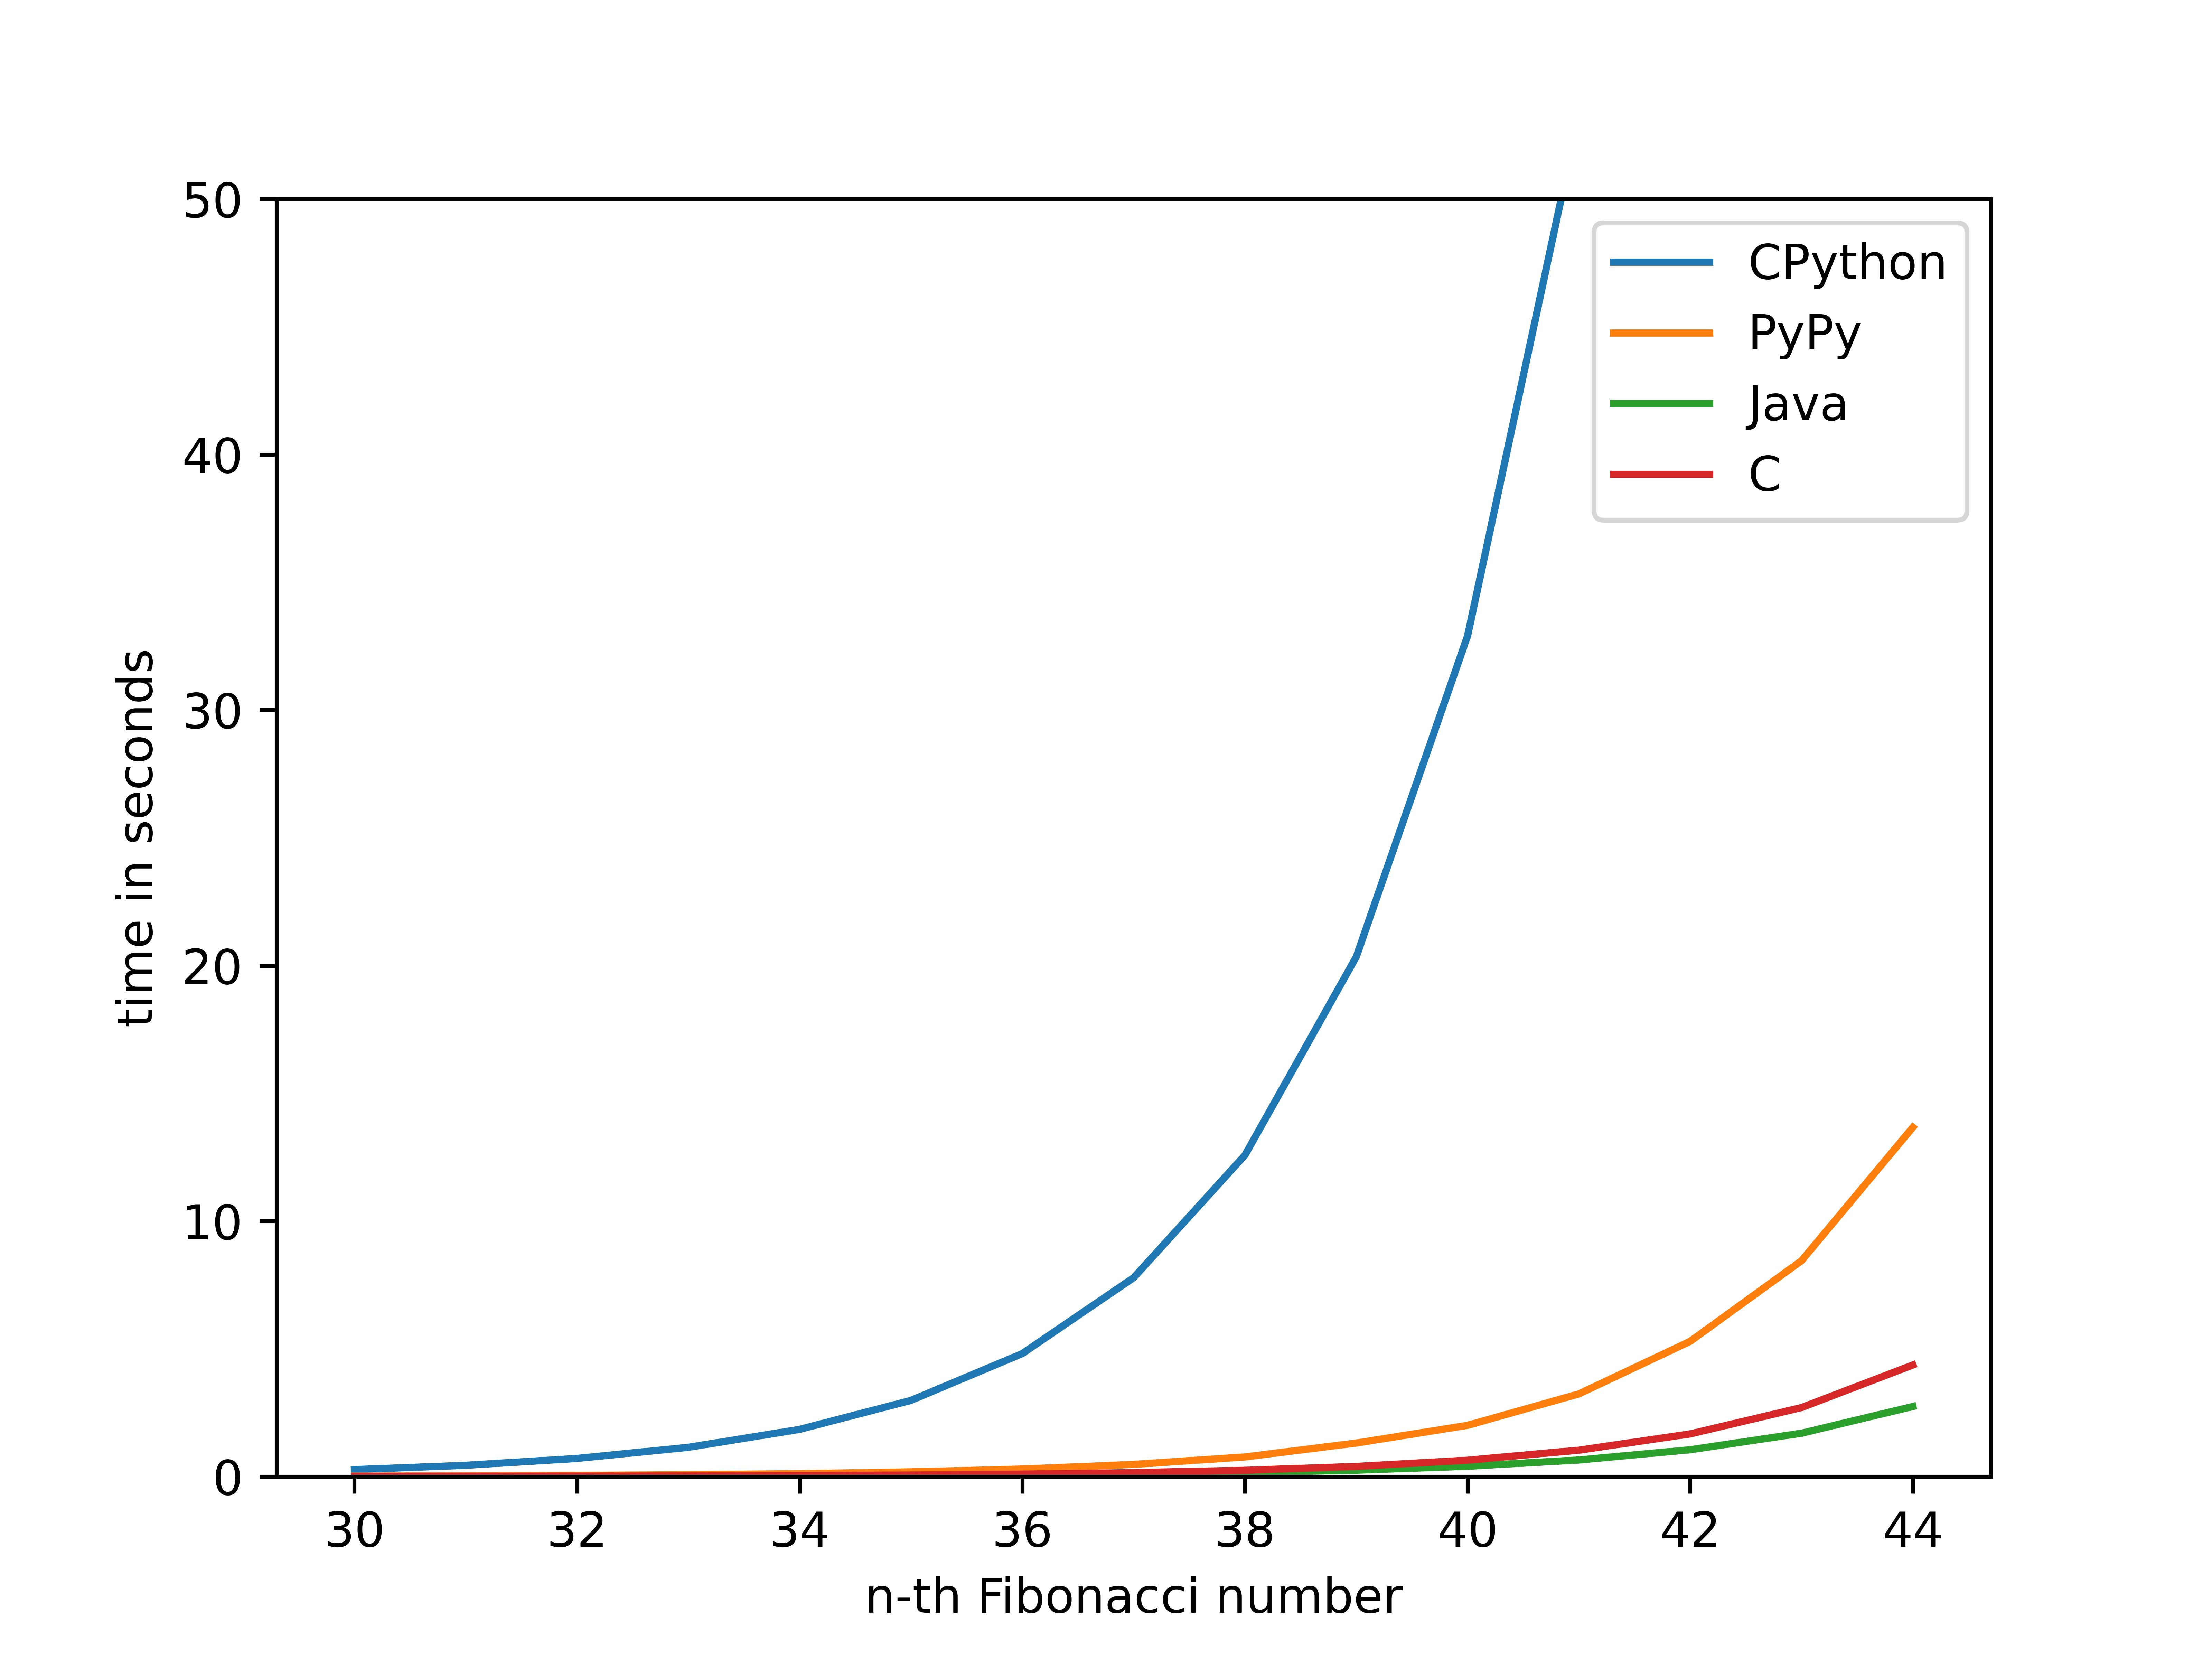
\includegraphics[scale=0.8,keepaspectratio]{images/lang_comparison.jpg}
\end{center}
\caption{Runtime comparison for recursive Fibonacci function.}
\label{fig:lang_comparison}
\end{figure}

We ran the test once using Python 3.9.16 with the packaged CPython interpreter and then with PyPy3.9, the equivalent PyPy release. Figure \ref{fig:lang_comparison} shows the results of this test. For every Fibonacci number, we ran the function 5 times, with the times shown being the averages of these 5 runs. Even from this basic example, the performance advantage of using PyPy over the CPython interpreter is apparent. For comparison, we also included the results for compiled languages like Java and C. Despite the significant time savings gained by using PyPy, it is still not as fast as compiled languages. However, we believe the existence of extensive graph libraries in the Python ecosystem outweighs this disadvantage.

\begin{figure}[H]
\begin{center}
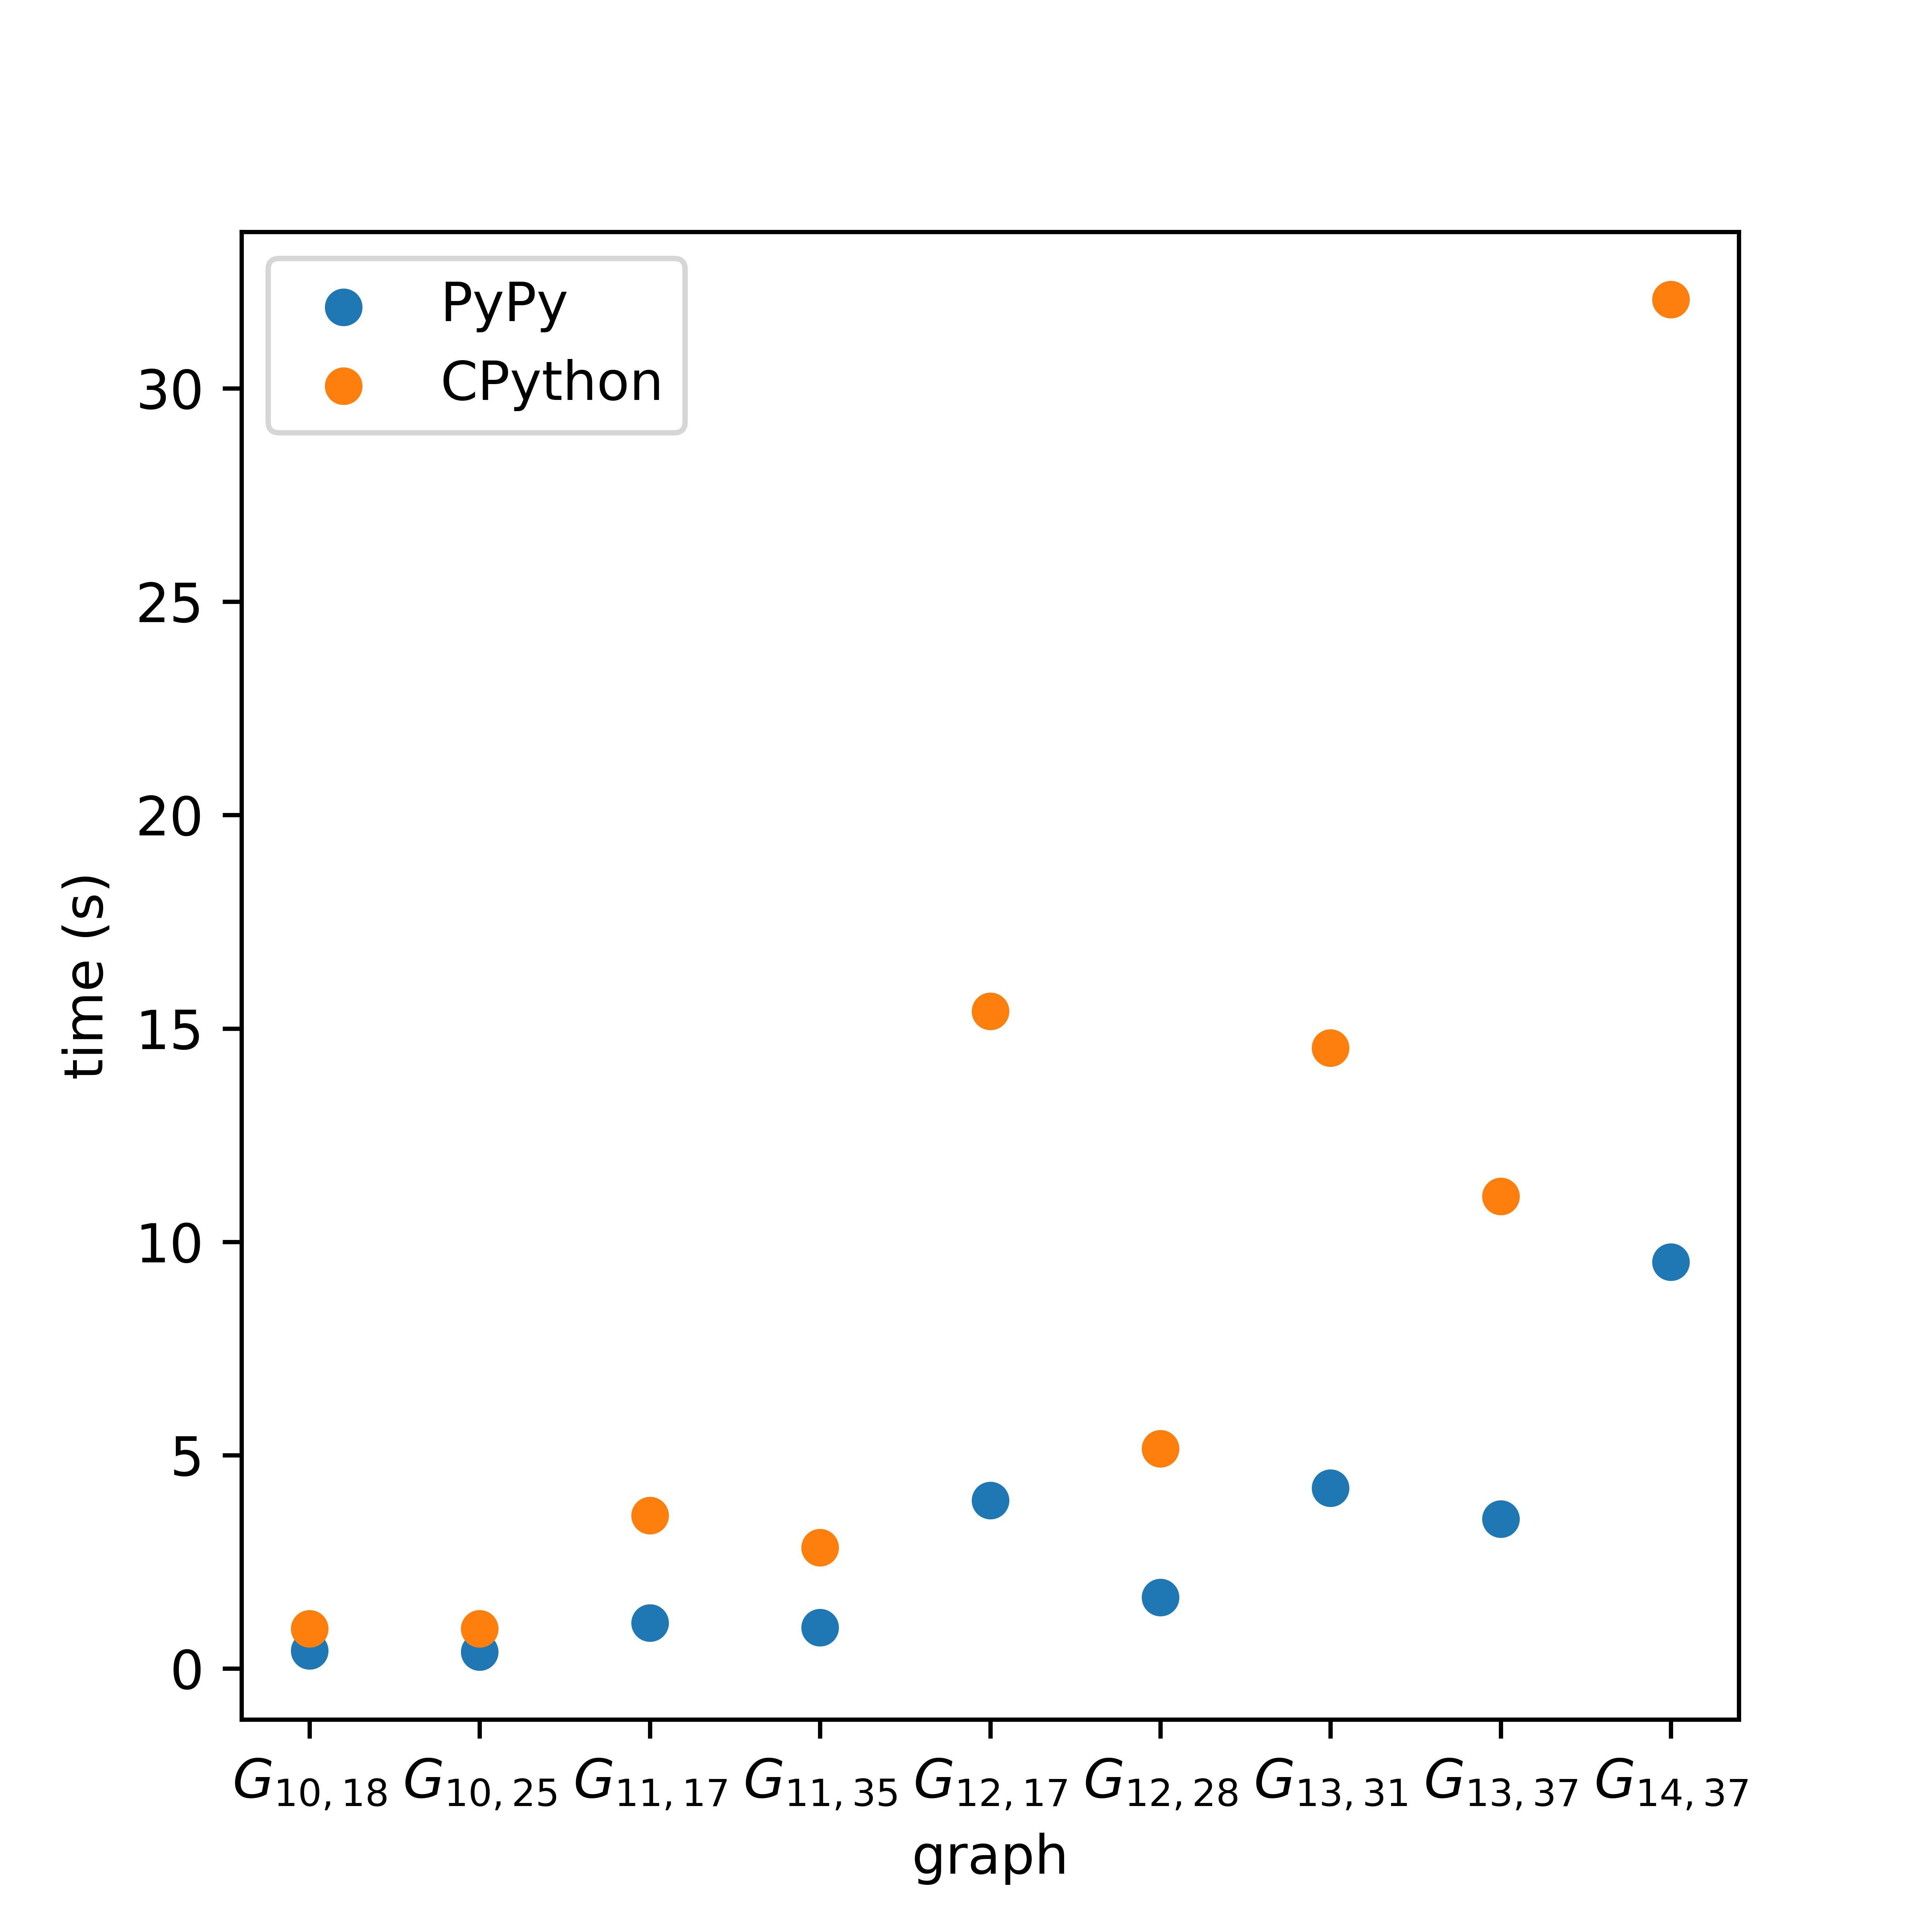
\includegraphics[scale=0.8,keepaspectratio]{images/cpython_pypy_comparison.jpg}
\end{center}
\caption{Runtime comparison of our algorithm for CPython and PyPy for graphs $G_{v,e}$, where $v$ is the number of vertices, and $e$ is the number of edges.}
\label{fig:cpython_pypy_comparison}
\end{figure}

To verify PyPy is indeed faster than CPython for our specific use case, we ran tests with our algorithm for finding the partial automorphism monoid. Results of this test are in Fig. \ref{fig:cpython_pypy_comparison}. PyPy achieved better performance in all test cases, and as expected, the difference got more significant for graphs with longer runtimes.

\subsection{Algorithm optimization}

While we achieved significantly better performance for our solution just by using a different interpreter, we took additional steps to improve the performance further.

We specifically focused on the process of finding isomorphism classes and their member for vertex-induced subgraphs. Our first version put the isomorphism classes into a list, so for every new subgraph, we had to traverse this list to check whether the graph is a member of any previously found isomorphism class, which resulted in many calls of the $is\_isomorphic$ function (isomorphism checks). In order to decrease the number of isomorphism checks, we used an isomorphism class filtering approach. We filter isomorphism classes by the degree sequences of their representatives. We create a dictionary in which the keys are degree sequences, and the associated values are isomorphism classes with that degree sequence.

When using the degree sequence filtering approach, we use the following process for every induced subgraph with degree sequence $ds$. We first check if a key $ds$ already exists in the dictionary. If not, we know this subgraph does not belong to any isomorphism class we found previously. If the key exists, we check whether the graph is isomorphic to the representative of any isomorphism class with the same degree sequence. In Python, searching for a key in a dictionary and adding a key gets done in $\mathcal{O}(1)$ time in an average case, making the approach especially effective for graphs that contain many unique degree sequences and graphs with many induced subgraphs \cite{dicttime}.

Our final improvement involved filtering the subgraphs using not only their degree sequence but also their \emph{triangle sequence}. We calculate the triangle sequence by calculating the number of triangles each vertex is a part of, where a triangle is a 3-clique, and sorting these numbers in ascending order. To calculate the number of triangles containing a given vertex $v$, we take the set of neighbors $N(v)$ and count how many vertices from unique 2-element subsets of $N(v)$ are connected with an edge.

In Table \ref{table:isomorphic_calls}, we can see the difference in the number of isomorphism checks between the version that does not filter the induced subgraphs, the version in which we filter them by their degree sequence, and finally, the version that filters not just by the degree sequence, but also by the triangle sequence.

A significant reduction in the number of isomorphism checks greatly decreased the time required to find isomorphism classes.

We included two graphs with 11 vertices and only 1 and 2 edges to observe cases in which the time saved using $dtf$ and $df$ is minimal compared to $nf$. Because these graphs are sparse, a vast majority of induced subgraphs of these graphs will have the same degree and triangle sequences. However, even in the case of graphs with 0 edges, the number of isomorphism checks will always be less for $dtf$ and $df$ approaches compared to $nf$. All graphs with less than five vertices having the same degree sequence (and consequently degree triangle sequence) are always isomorphic, so we need no isomorphism checks for induced subgraphs with less than five vertices. While we decrease the number of isomorphism checks, the cost of calculating the degree sequence or triangle sequence is comparable to the cost of an isomorphism check, so the runtime is very similar.

In some of the remaining cases, we see a significant decrease in the number of isomorphism checks when using graph filtering as well as a substantial decrease in the runtime. In the case of the 16 vertex graph with 84 vertices ($\delta = 0.7$), $dtf$ decreased the number of isomorphism checks by more than 99\%, while the runtime decreased by 83\%. On the other hand, in the case of a graph with 14 vertices and a density of 0.82, the difference was less noticeable than in the earlier case. While we still decreased the number of isomorphism checks by more than 98\%, the time saved was only 9.3\%.

\begin{figure}[H]
\begin{center}
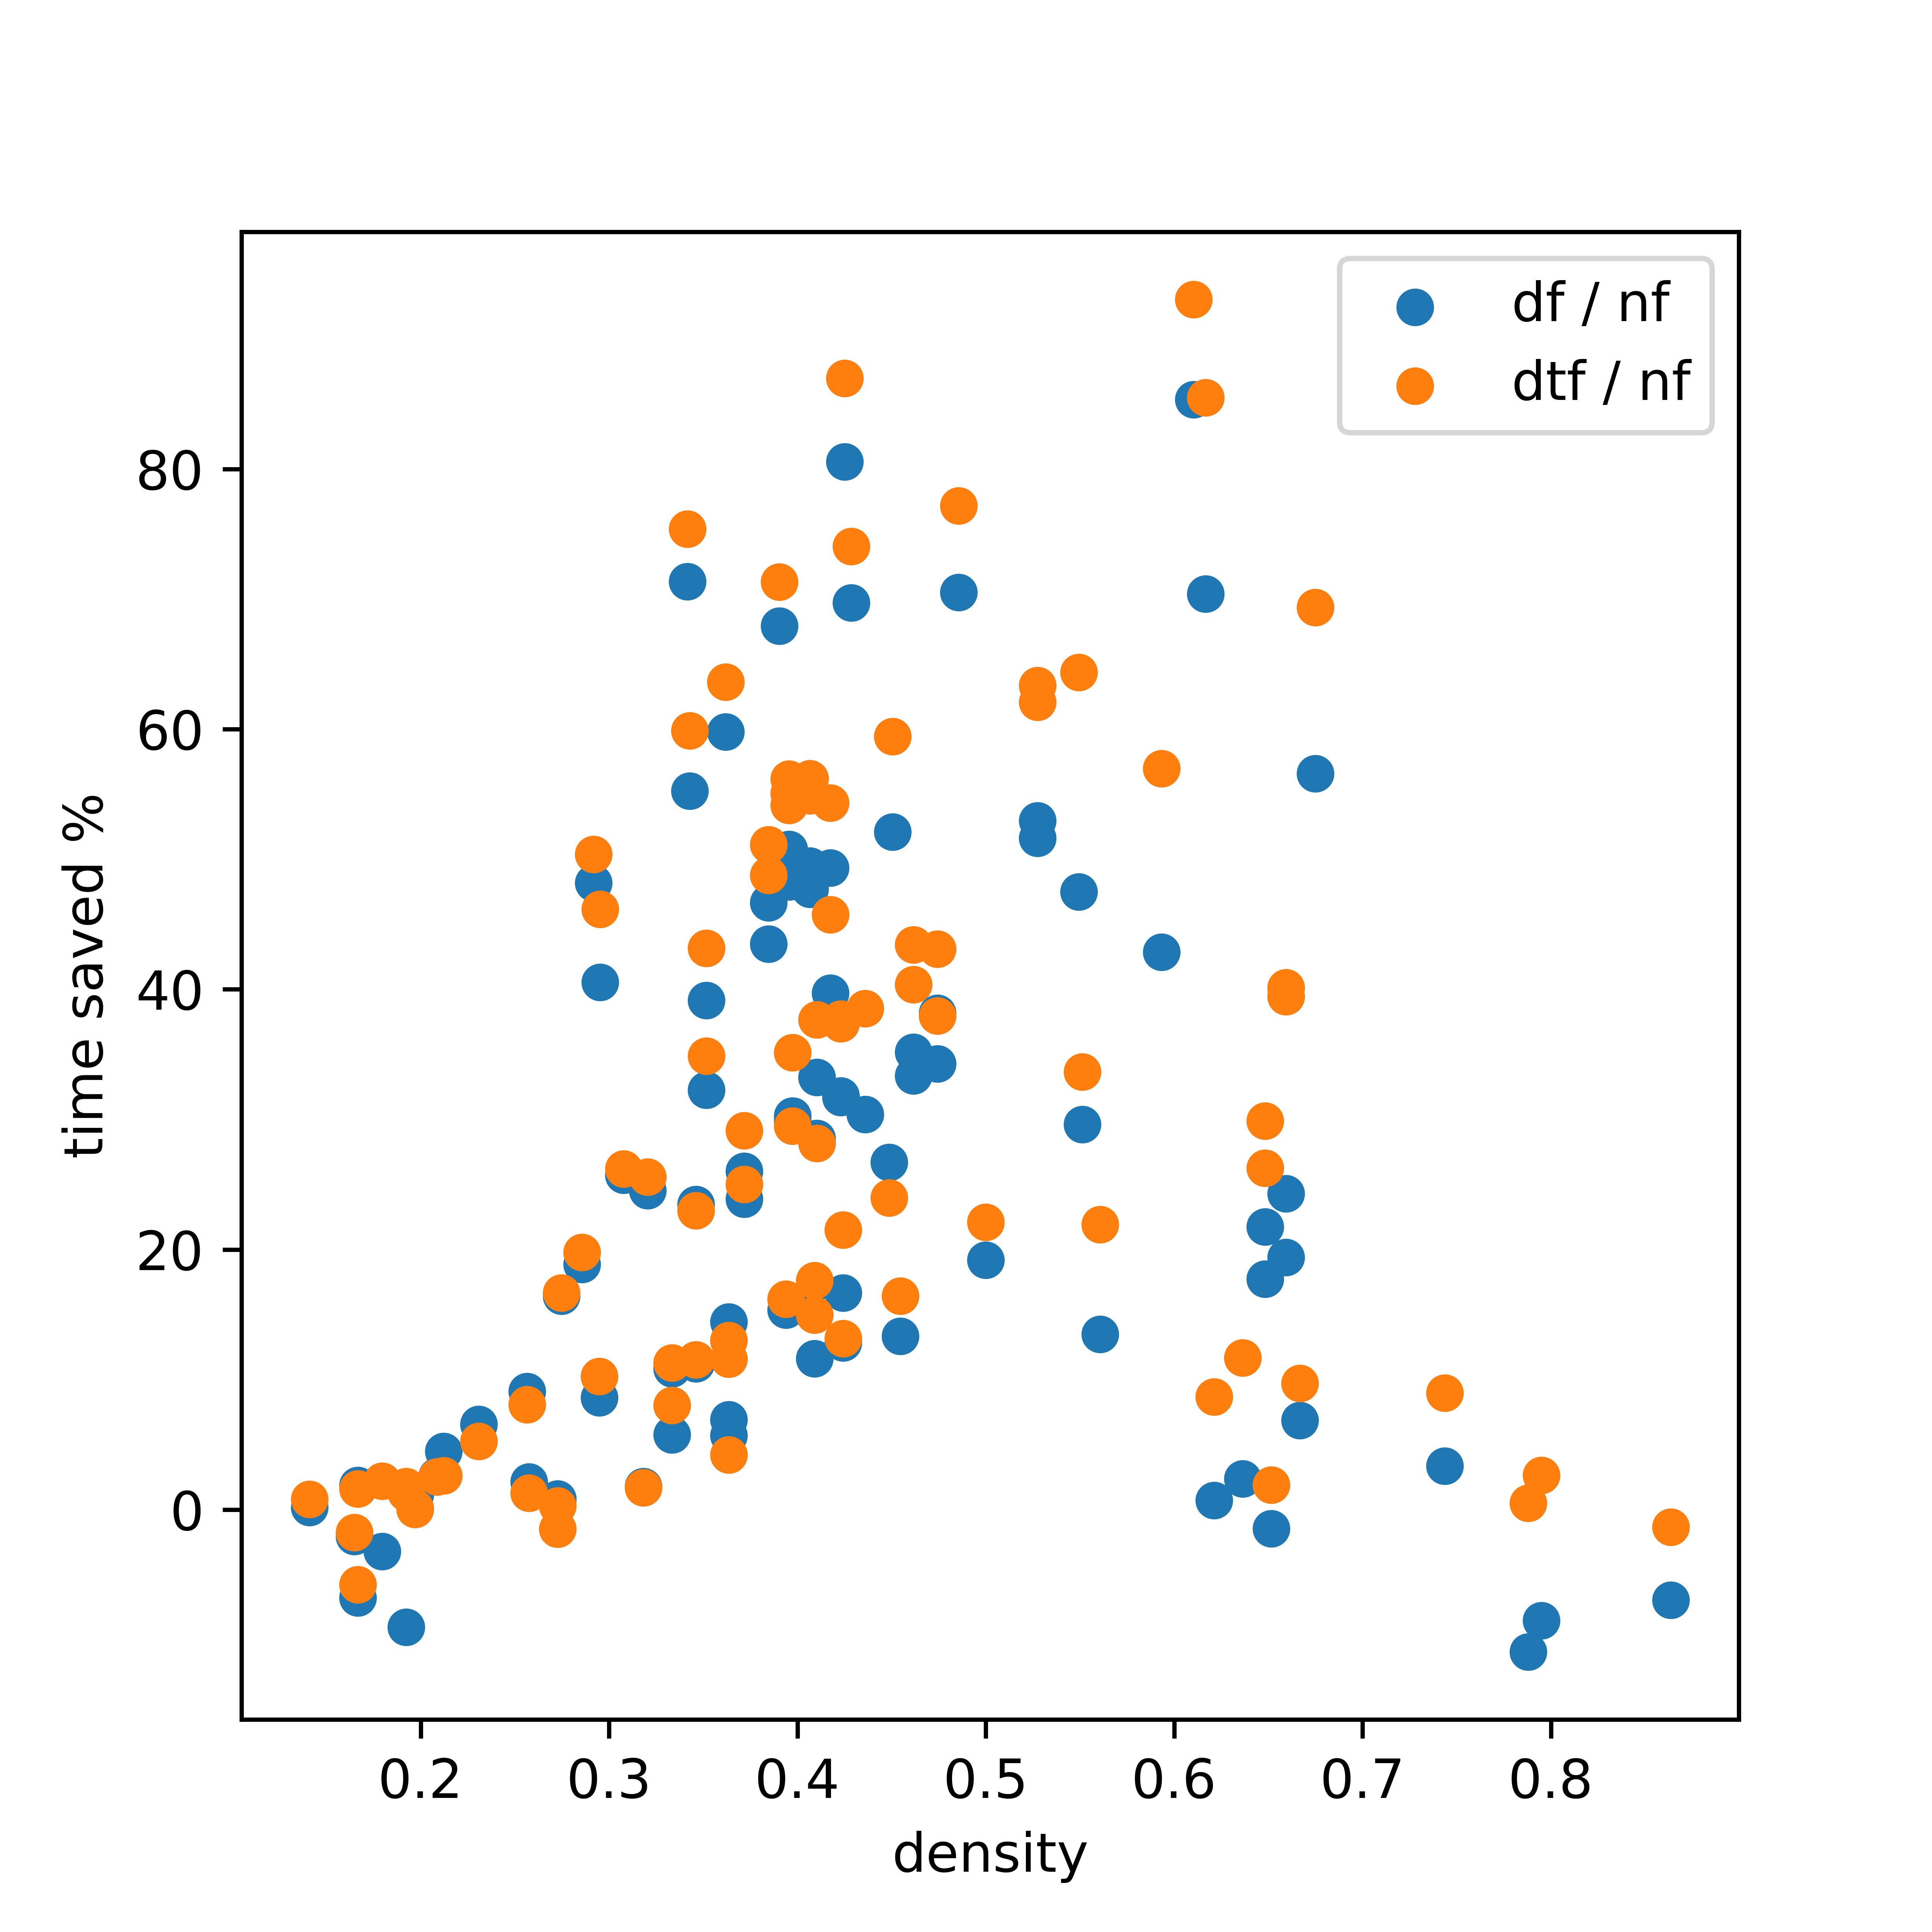
\includegraphics[scale=0.8,keepaspectratio]{images/density_filter_type_comparison.png}
\end{center}
\caption{Comparison of the time saved when using $dtf$ and $df$ graph filtering approaches compared to no filtering ($nf$).}
\label{fig:filter_type_comparison}
\end{figure}

In conclusion, the time we can save by filtering the graphs by their degree sequences or degree triangle sequences depends on the graph's structure. The time saved will be less for sparse graphs or their complements, dense graphs. The time saved will be the greatest for graphs with many unique degree and triangle sequences, which causes a significant drop in the number of isomorphism checks compared to no filtering approach. Generally, the $df$ and $dtf$ should perform significantly better for graphs with density $\delta = 0.5 \pm 0.3$.

To verify these claims, we ran tests on randomly generated graphs with 12+ vertices, with the results shown in Fig. \ref{fig:filter_type_comparison}. For some sparse graphs with a density of less than 0.2 and dense graphs with a density of at least 0.8, the sequence filtering approaches might be slower when compared to the no-filtering approach. Meanwhile, graph filtering performs better in the remaining cases, with a few exceptions.

\begin{table}
\begin{tabular}{ | c | c | c | c | c | c | c | c | }
\hline
\multicolumn{2}{|c|}{Graph info} & \multicolumn{6}{c|}{Filter type} \\
\hline
|V(G)| & |E(G)| & $nf$ & t(s) & $df$ & t(s) & $df$ + $dtf$ & t(s) \\
\hline
11 & 1 & 2514 & 74.024 & 1473 & 72.961 & 1473 & 71.714 \\
11 & 2 & 3028 & 39.448 & 1467 & 38.732 & 1467 & 39.053 \\
14 & 75 & 822268 & 70.703 & 18619 & 67.952 & 13763 & 64.088 \\
15 & 64 & 24511511 & 84.855 & 176682 & 24.324 & 20380 & 9.337 \\
15 & 76 & 11915998 & 61.482 & 94851 & 31.661 & 23577 & 17.083 \\
15 & 84 & 3959678 & 72.918 & 68546 & 63.032 & 27091 & 42.625 \\
16 & 84 & 56858121 & 247.703 & 295276 & 99.501 & 47644 & 41.821 \\
\hline
\end{tabular}
\caption{\label{table:isomorphic_calls} Comparison between the number of isomorphism checks when using different induced subgraph filtering approaches ($nf$ - no filter, $df$ - degree sequence filter, $dtf$ - degree triangle sequence filter).}
\end{table}

\section{Web Application}
\label{sec:web}

Some other theses that dealt with graphs and their automorphisms used a simple command line interface. We decided against this approach since command-line applications are generally difficult to work with. For example, in the case of manually entering a graph, if the user makes a mistake, they are required to re-enter the entire graph again. Also, displaying larger automorphisms or partial automorphism monoids in the command line with basic text graphics is confusing.

Therefore, in order to make the application more user-friendly, we created a dynamic single-page web application. On the frontend, we worked in the Vue.js ecosystem, using Vue Router for routing, Pinia for page-wide storage, and Vuetify for design \cite{vue, pinia, vuetify}. On the backend, we used Django, a Python web framework, and Django Rest framework, a framework for creating REST APIs \cite{django, drf}. The backend-frontend communication gets handled using Axios, and the data exchanged is in JSON format \cite{axios}.

\subsection{Minimal assymetric graphs}

The home page of the web page is dedicated to the primary goal of this thesis, minimal asymmetric graphs and their partial symmetries. Users can select which minimal asymmetric graph's symmetries they want to view in a simple drop-down list. The partial symmetries are then loaded and displayed to users. The structure of the partial automorphism monoid is displayed at the top of the page, as shown in Fig. \ref{fig:website_monoid_structure}. It illustrates the structure of the partial automorphism monoid but also serves as a navigation, where users can scroll to a $\mathcal{D}$-class of a given induced subgraph by clicking the appropriate button. How $\mathcal{D}$-classes are displayed on the website is shown in Fig. \ref{fig:website_d_class}. Above the $\mathcal{D}$-class is a visualization of a representative of the isomorphism class, generated using the $pyvis$ library. Vertices in the visualization can be dragged, and users can zoom in or out on parts of the graph. Users can get additional information about the elements on the main diagonal, that contain idempotents and form a group, by clicking the information icon.

\begin{figure}[H]
\begin{center}
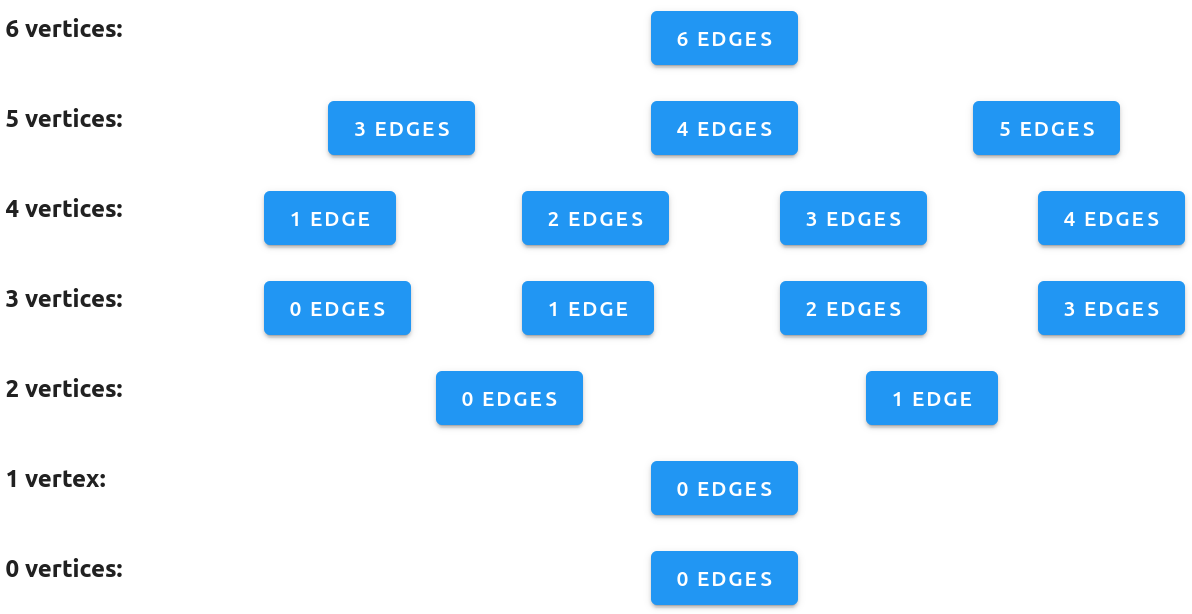
\includegraphics[width=\textwidth,keepaspectratio]{images/website_monoid_structure.png}
\end{center}
\caption{An example of how the structure of the partial automorphism monoid gets displayed on the webpage.}
\label{fig:website_monoid_structure}
\end{figure}

\begin{figure}[H]
\begin{center}
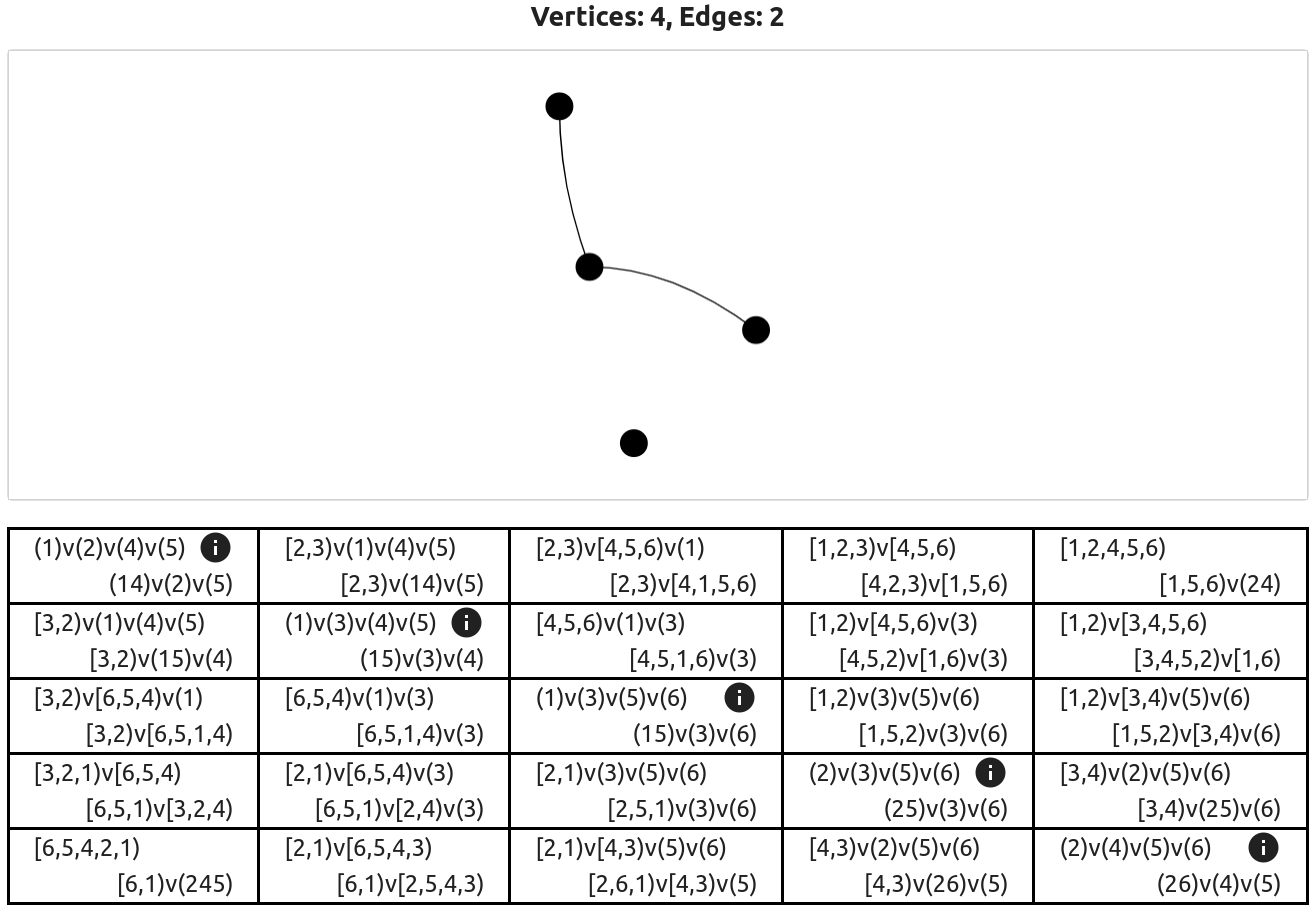
\includegraphics[width=\textwidth,keepaspectratio]{images/website_d_class.png}
\end{center}
\caption{An example of the $\mathcal{D}$-class for an isomorphism class.}
\label{fig:website_d_class}
\end{figure}

\subsection{Custom graphs}

We also created a page for users to enter custom graphs in an easy-to-use interface. Users can select the number of vertices of a graph in a slider, with the maximum amount of vertices set to 10. The reason for setting the limit at 10 is the exponential increase in the number of partial symmetries. For example, 10-vertex graphs might have more than a million partial symmetries. Limiting the web page to smaller graphs also decreases the server load and the amount of data exchanged between the server and the client.

For every vertex, users can enter the set of neighbors of this vertex by selecting vertices in a multi-select element. Since the graphs used by our application are undirected, once the user selects vertex $u$ to be the neighbor of vertex $v$, the vertex $v$ gets set automatically as the neighbor of vertex $i$. After the user updates the set of neighbors for any vertex, a visualization of a graph based on the current values is displayed.

\begin{figure}[H]
\begin{center}
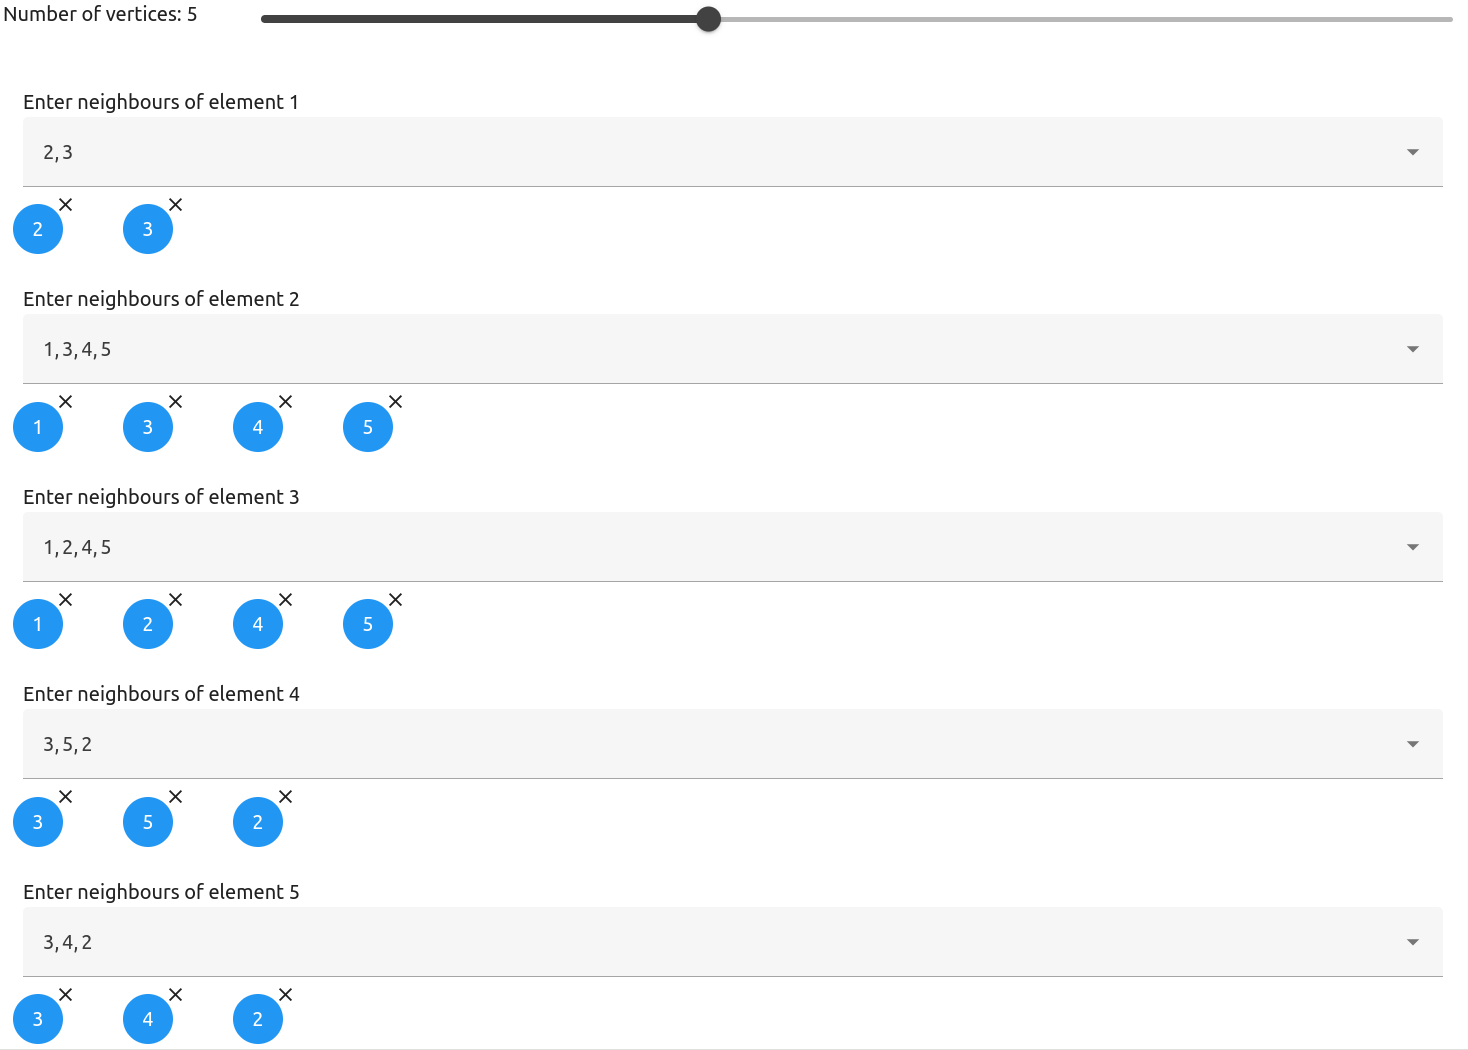
\includegraphics[width=\textwidth,keepaspectratio]{images/website_custom_graph.png}
\end{center}
\caption{Custom graph creation component.}
\label{fig:website_custom_graph}
\end{figure}
